

\subsection{Spin coherence time requirements}
Operating in the space domain FS methodological framework in a perfectly-aligned lattice,~\footnote{In fact,
perfect element alignment is a pre-requirement of the space domain.}
the spin coherence time (SCT) is determined by the minimal detectable angle
by which the polarization vector deviates from the beam orbit plane as a result of the EDM action
alone. For the sensitivity level of $10^{-29}~e\cdot cm$ this angle is approximately
$5\cdot10^{-6}$.~\cite{BNL:Deuteron2008}

According to the T-BMT equation,
\[
\W_{EDM,x} = \eta\frac{qE_x}{2mc},
\]
where $\eta$ is the proportionality coefficient between the EDM and spin,
in the deuteron case equal to $10^{-15}$, for the given sensitivity level.~\cite[p.~206]{Eremey:Thesis}

For the deuteron BNL FS ring, $E_x = 12$
MV/m,~\cite[p.~19]{BNL:Deuteron2008} therefore $\W_{EDM,x}\approx 10^{-9}$ rad/sec.
Hence we obtain that, in order to reach a detectable level of at least 1 $\mu$rad one needs an SCT
on the order of 1,000 seconds.~\cite[p.~207]{Eremey:Thesis}
\subsection{Origins of decoherence}\label{sec:decoh:origin}
Spin decoherence in a particle beam results from the dispersion of the beam particles'
spin precession angular velocities, which, in its turn, is a result of the difference
between their orbit lengths and initioal momenta. The orbit length effect on the particle spin tune
is described by the concept of the effective Lorentz-facotr, which was introduced
in section~\ref{chpt1:FS-methods:effective-Lorentz-factor}.

Frim equations~\eqref{eq:spin_tune_vs_gamma} for spin tune in electrostatic and magnetic fields it follows that 
the spin tunes of two particles having equal values of the effectove L-factor are equal, regardless of
their trajectories in the accelerator. This principle is the basis for the proposed sextupole field
spin precession suppression theory, as well as the procedure for flipping the polarity of the storage ring's
guide field, which is required for injecting the deuteron beam in the opposite direction in order to cancel
the EDM-faking MDM spin precession.

\subsection{Sextupole field spin decoherence suppression theory}\label{sec:sextupole_spin_dec_solution}
In order to minimize spin decoherence related to particle betatron motion and momentum spread
sextupole (or octupole) fields can be used.~\cite[p.~212]{Eremey:Thesis}

A sextupole of strength
\[
S_{sext} = \frac{1}{B\rho} \pddx{B_y}[x][2],
\]
where $B\rho$ is the magnetic rigidity, modifies the first-order momentum
compaction factor as~\cite[p.~2581]{Senichev:IPAC13}
\begin{align}
	\Delta \alpha_{1,sext} &= -\frac{S_{sext}D_0^3}{L}, \label{eq:Sext_compaction_effect}
	\intertext{and simultaneously the orbit length as}
	\bkt{\frac{\Delta L}{L}}_{sext} &= \mp \frac{S_{sext}D_0\beta_{x,y}\varepsilon_{x,y}}{L}, \label{eq:Sext_OL_effect}
\end{align}
where $D(s,\delta) = D_0(s) + D_1(s)\delta$ denotes the dispersion function.

One can formulate the principle of the sextupole field effect in the following way.
A particle in an accelerator does performs betatron oscillations about some closed orbit.
Due to dispersion, the closed orbit is different for different particles in the beam.
A sextupole field works like a prism, focusing (or defocusing) the praticles' closed orbits.

In the next sections we will call the decoherence associated with the horizontal/vertical
betatron oscillations, respectively synchrotron oscillations, the X-/Y-, and D-decoherence.
Sextupole families aimed at reducing X-, Y-, and D-decoherence will be denoted, respectively,
GSX, GSY, GSD.

From equations~\eqref{eq:Sext_compaction_effect}, and~\eqref{eq:Sext_OL_effect} one can
see that one needs to use three sextupole families, placed respectively
in the maxima of the $\beta_x$, $\beta_y$ (for the X-,Y-types), and
$D_0$ (for the D-type) functions, in order to suppress spin decoherence in the beam.

\subsection{Simulation in an ideal ring}\label{sec:decoh:suppression_in_ideal_lattice}

In order to check the capability of the sextupole field spin decoherence suppression method we
carried out a simulation in which we used the FS-type lattice described in section~\ref{chpt2:lattice:FS_BNL}.
Since the lattice is perfectly aligned, spin precession occurs only about the vertical ($\hat y$) axis. 

SCT optimization is done at 270.00 MeV enegrgy, the orbital and spin transfer matrices of the lattice
are computed up to the fifth order of the Taylor expansion.

Three sextupole families are used, to suppress the X, Y-, and D-type decohrence respectively.
Each sextupole family's field gradient is optimized separately (the gradients of the other two
families are set to zero). We optimize the sextupoles separately because otherwise we run into a
numerical problem with the TSS procedure.~\footnote{We also studied the possibility of finding the optimal
  set of gradient values, by directly computing the relevant spin tune Taylor expansion coefficients in the
  3D gradient space mesh. The question needs further investigation, but at this point we doubt that all
  three families can be optimized simultaneously. This could be the reason why in~\cite[p.~219]{Eremey:Thesis}
  only two sextupole families are used in the lattice codenamed BNL.}

The sextupole field optimization procedure is as follows. First, the lattice's
transfer matrices are computed at the given sextupole gradient strength. Then, using procedure TSS
we compute the spin tune and invariant spin axis (ISA) Taylor expansions. Depending on the optimized family,
we pick the coefficient at the square of the corresponding phase space variable ($x$, $y$, or $\delta$)
from the spin tune Taylor expansion. The absolute value of the coefficient is used as the objective
function: i.e., at the optimal gradient, does not depend (parabolically) on the corresponding
particle offset from the reference one.

The Simplex algorithm was used for optimization.~\cite[p.~37]{COSYINF:Manual:Programmer}

In Figure~\ref{fig:decoh:perfect} the spin tune dependence on the particle offset from reference in three
phase space coordinate before and after turning on the relevant sextupoles. One can see that in all
three cases the parabolic dependence has been suppressed. However, there remains a linear dependence,
which is insensitive to the sextupole fields. The linear dependence is observed when modeling the spin
dynamics in the codes COSY INFINITY, MODE, as well as MAD (from private communication with Y. Senichev).
Based on that, one can hypothesize that the linear term is not a numerical artifact of  COSY INFINITY,
but rather has a physical basis. This question needs further consideration, but at this point it is thought that
this term can be suppressed by adjusting the RF cavity parameters.~\cite[p.~210,~219]{Eremey:Thesis}

\begin{figure}[!h]
	\centering
	\begin{subfigure}{\linewidth}
		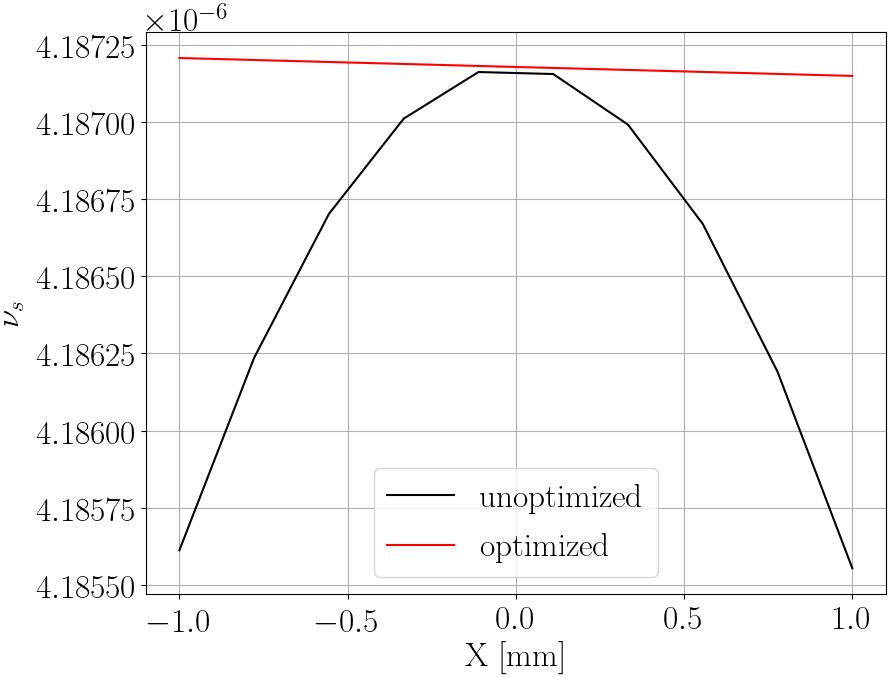
\includegraphics[height=.35\paperheight]{images/decoh_sim/spin_tune_decoh_x_offset}
		\caption{Radial offset}
	\end{subfigure}
	\begin{subfigure}{\linewidth}
		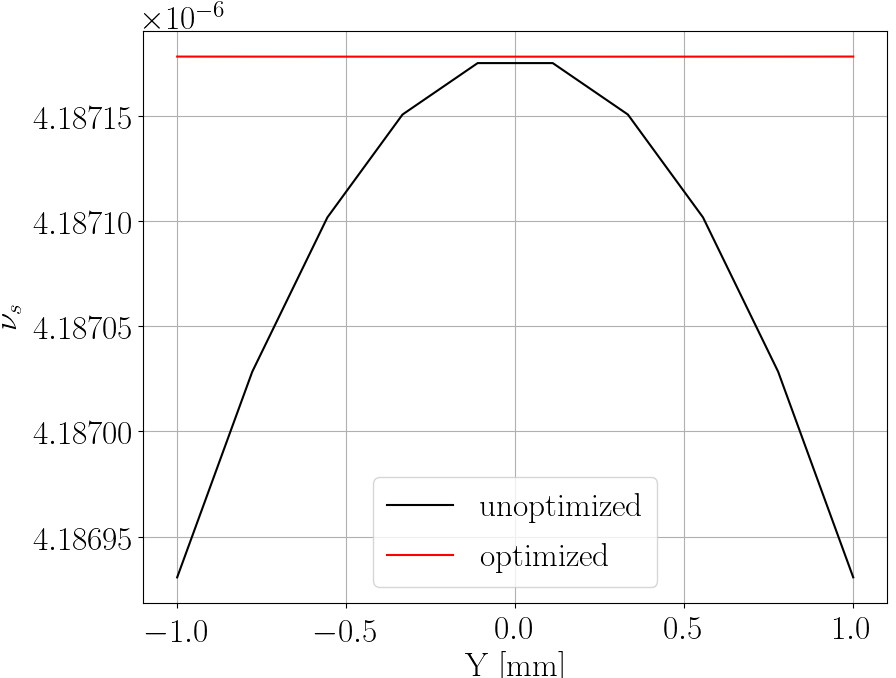
\includegraphics[height=.35\paperheight]{images/decoh_sim/spin_tune_decoh_y_offset}
		\caption{Vertical offset}
	\end{subfigure}
\end{figure}
\begin{figure}[!h]\ContinuedFloat\centering
	\begin{subfigure}{\linewidth}
		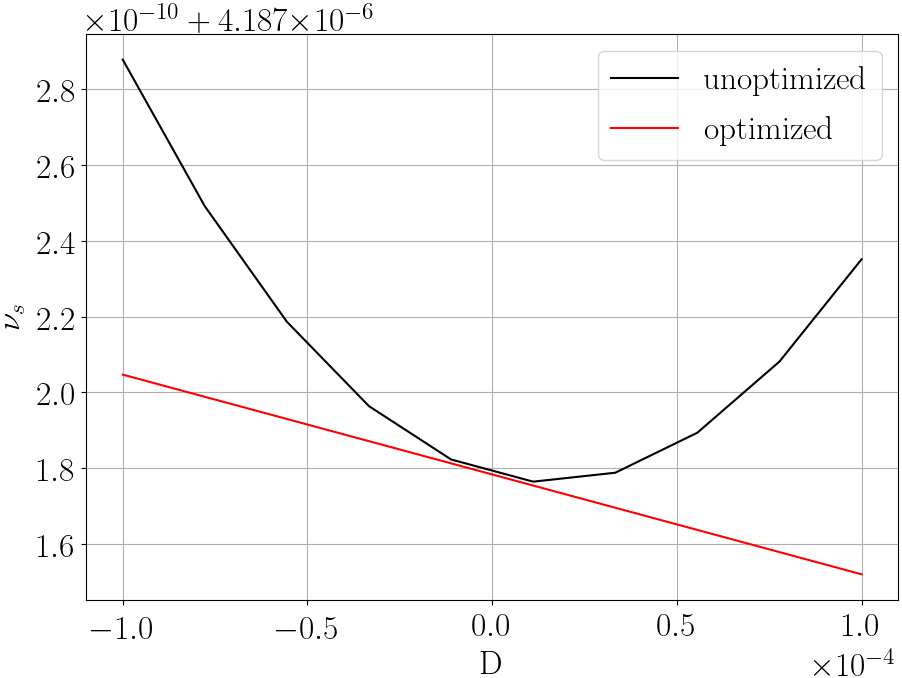
\includegraphics[height=.35\paperheight]{images/decoh_sim/spin_tune_decoh_d_offset}
		\caption{Energy offset}
	\end{subfigure}
	\caption{The dependence of a particle spin tune on its initial offset
          from the reference particle.\label{fig:decoh:perfect}}
\end{figure}

\subsection{Transfer of decoherence into the vertical plane in an imperfect lattice}
We injected an ensemble of 30 particles, uniformly distributed along the vertical axis in the range
$y \in [-1, +1]$ mm, into an imperfect FS lattice. Since the analysis is based only on the tracker data,
and does not involve the TSS procedure, the beam was injected at the exact FS energy 270.0092 MeV.

Imperfections are simulated by E+b element tilts about the optic axis by angles picked from the normal
distribution $\Theta_{tilt} \sim N(0, 1\cdot 10^{-4})$ radians. Since such imperfections conserve the
Lorentz force, they do not perturb the particle orbital dynamics and affect only the spin dynamics.
The magnitude of the standard deviation reflects the realistic element alignment precision.

In Figure~\ref{fig:decoh:SX_SD} we show the standard deviation of the radial components of
the ensemble's spin vectors before and after turning on the sextupoles.
Since the particles move in an imperfect lattice, their spin vectors rapidly turn in the vertical plane,
and hence $\sigma_{s_x}$ is a rapidly oscillating function exhibiting no long-term growth trend
(the slope of the trend line is $(2\pm2)\cdot 10^{-8}$ 1/sec). This means there's no spin decoherence
in the horizontal plane. When the sextupoles are turned on the $\sigma_{s_x}$ amplitude is reduced by
a factor of 10.

In Figure~\ref{fig:decoh:SY_SD} is shown the same statistic for the vertical spin vector components.
A long-term trend is observed (the slope is $(4.5 \pm 0.6)\cdot 10^{-7}$ 1/sec) prior to turning on
the correcting sextupoles. The sextupole correction does not reduce the oscillation amplitude, 
but suppresses the accummulation of dispersion (the slope drops to $(5\pm 6)\cdot 10^{-8}$ 1/sec).

\begin{figure}[h!]
	\centering
	\begin{subfigure}{\linewidth}
		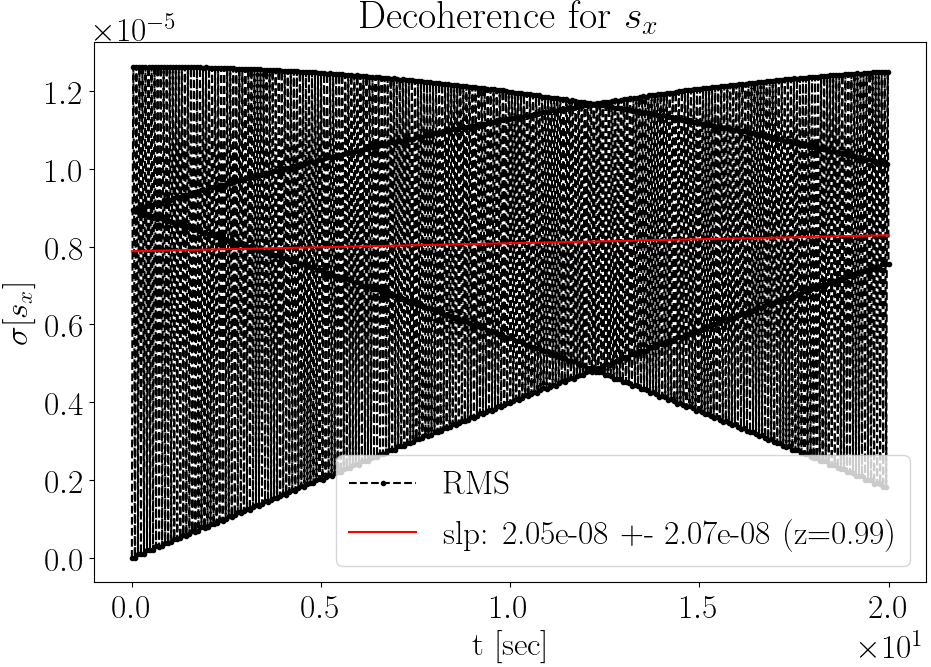
\includegraphics[height=.35\paperheight]{images/decoh_sim/SX_decoh_20sec_unopt}
		\caption{Sextupoles off}
	\end{subfigure}
	\begin{subfigure}{\linewidth}
		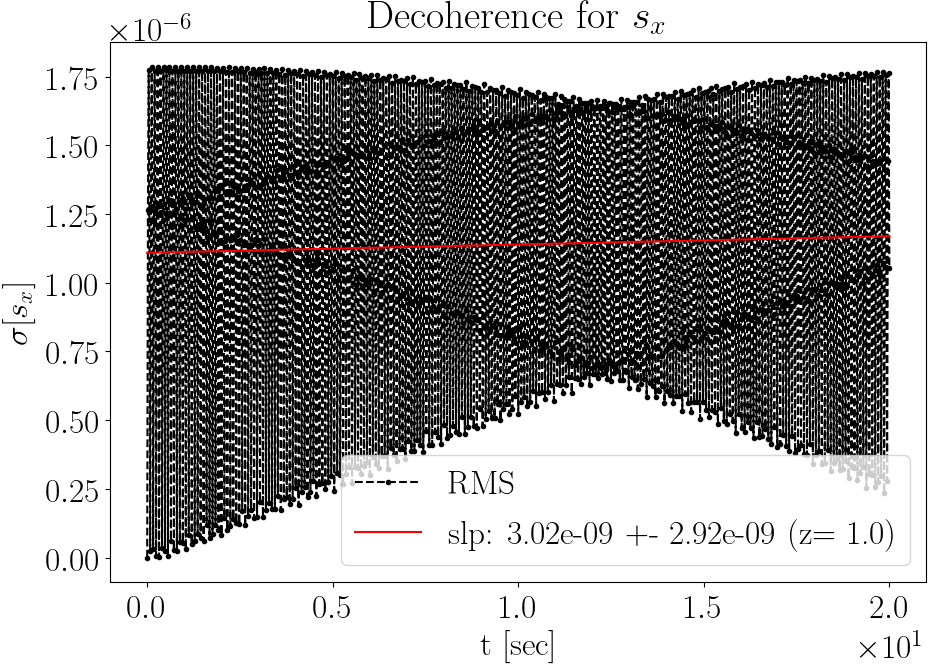
\includegraphics[height=.35\paperheight]{images/decoh_sim/SX_decoh_20sec_opt}
		\caption{Sextupoles on}
	\end{subfigure}
	\caption{Standard deviation of the radial spin vector component distribution in a bunch.\label{fig:decoh:SX_SD}}
\end{figure}

\begin{figure}[h!]
	\centering
	\begin{subfigure}{\linewidth}
		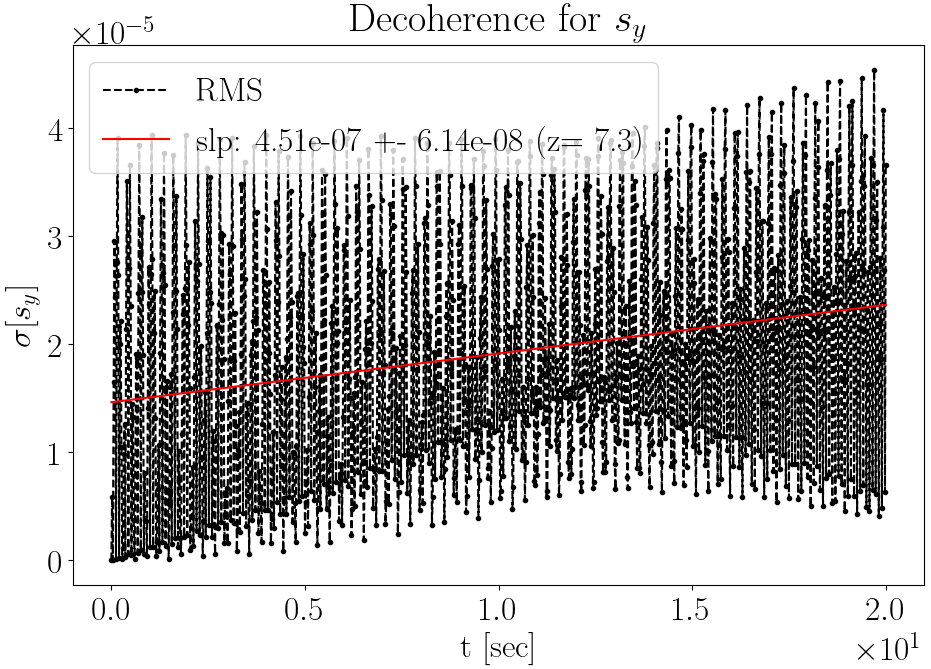
\includegraphics[height=.35\paperheight]{images/decoh_sim/SY_decoh_20sec_unopt}
		\caption{Sextupoles off}
	\end{subfigure}
	\begin{subfigure}{\linewidth}
		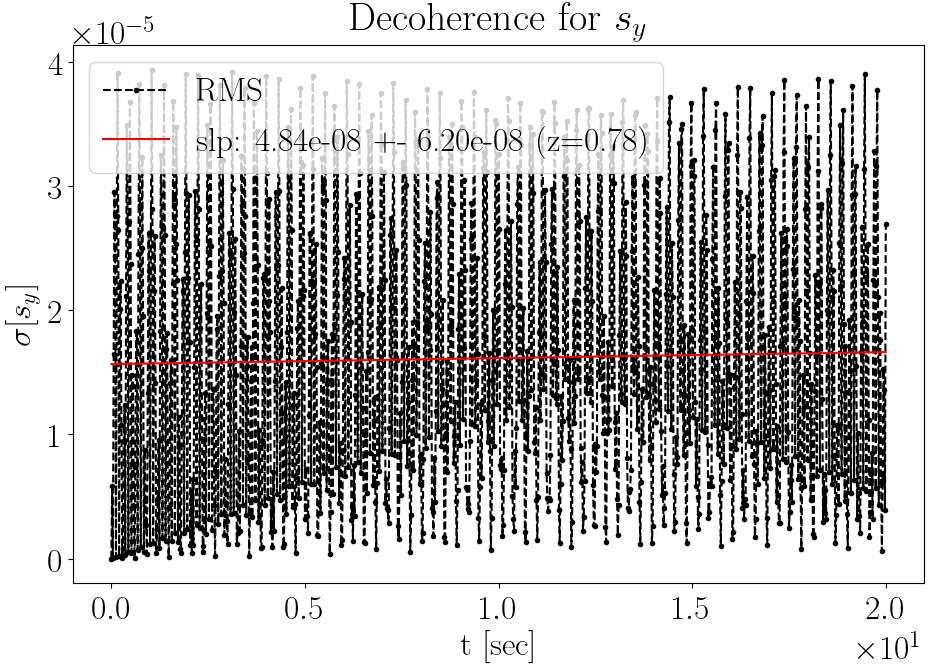
\includegraphics[height=.35\paperheight]{images/decoh_sim/SY_decoh_20sec_opt}
		\caption{Sextupoles on}
	\end{subfigure}
	\caption{Standard deviation of the radial spin vector component distribution in a bunch.\label{fig:decoh:SY_SD}}
\end{figure}

\subsection{Analysis of spin decoherence in an imperfect lattice}\label{sec:decoh:sim-imperfect}
The following tests were done with a planar bunch of 30 particles injected into a FS lattice
with E+B elements tilted about the optic axis by angles picked from $N(0, 5\cdot10^{-4})$ radians.

The beam particles were normally-distributed in the vertical plane $y-z$ along the $\hat y$-axis
as $y\sim N(y_0, 0.1)$ mm (all other phase space coordinates are zero). The offset $y_0$ varied in the
range $[-1, +1]$ mm. Initially all particles' spins were longitudinally oriented $\vec S(t=0) = (0,0,1)$.

We also varied the value $G_Y$ of the GSY sextupole.
$G_Y$ varied in the range $[G_Y^0 - 5\cdot10^{-3}, G_Y^0 + 5\cdot10^{-3}]$, where
$G_Y^0=-5.77\cdot 10^{-4}$ is the optimal gradient for this particular imperfection distribution.
The value $G_Y^0$ was found by minimizing the coefficient $a_2$
of the Taylor expansion $\nu_s(y) \approx a_0 + a_1\cdot y + a_2\cdot y^2 + O(y^3)$.

There were 10 injections at each value of $G_Y$.

To ensure the stability of the TSS procedure of COSY Infinity~\cite{COSYINF:Manual:BeamPhys},
the beam was injected at 270 MeV (the strict FS occurs at 270.0092 MeV), and the orbital and
spin transfer matrices were built up to the third order Taylor expansion. 

After that the beam is tracked through the lattice for $1.2\cdot10^6$ turns, which is approximately
equivalent to 1.2 seconds. Data used in the analysis were collected every 800 turns.

What we collected:
\begin{enumerate*}[\itshape a\upshape)]
	\item TSS procedure results: spin tune ($\nu_s$)  and the ISA ($\bar n$) components, and
	\item spin $(S_X, S_Y, S_Z)$ and phase space $(X,A,Y,B,T,D)$ vector components.
\end{enumerate*}
We also recorded the Taylor expansions of $\nu_s$, $\nbar$, orbital, and spin transfer matrices
of the lattice at each $G_Y$ value.

From the spin vector component data we computed the ensemble polarization:
\begin{equation}\label{eq:polarization_formula}
\vec P = \frac{\sum_i\vec s_i}{|\sum_i\vec s_i|}.
\end{equation}

Its vertical component is fitted by $f(t; a,f,\phi) = a\cdot \sin(2\pi\cdot
f\cdot t + \phi)$, where all three parameters $(\hat a, \hat f, \hat\phi)$ are estimated.  

\subsubsection{Sextupole field effect on spin tune and invariant spin axis}
In Figure~\ref{decoh:fig:ST_vs_y0_GSY} we showed the dependence of spin tune on the particle's
vertical offset from the reference orbit: $\nu_s(y) \approx a_0 + a_1\cdot y + a_2\cdot y^2 + O(y^3)$.
In Figure~\ref{decoh:fig:full:ST_vs_y0_GSY} one can observe the unbending of the parabola when
$G_Y \rightarrow G_Y^0$.
\begin{figure}[h!]
	\centering
	\begin{subfigure}{\linewidth}
		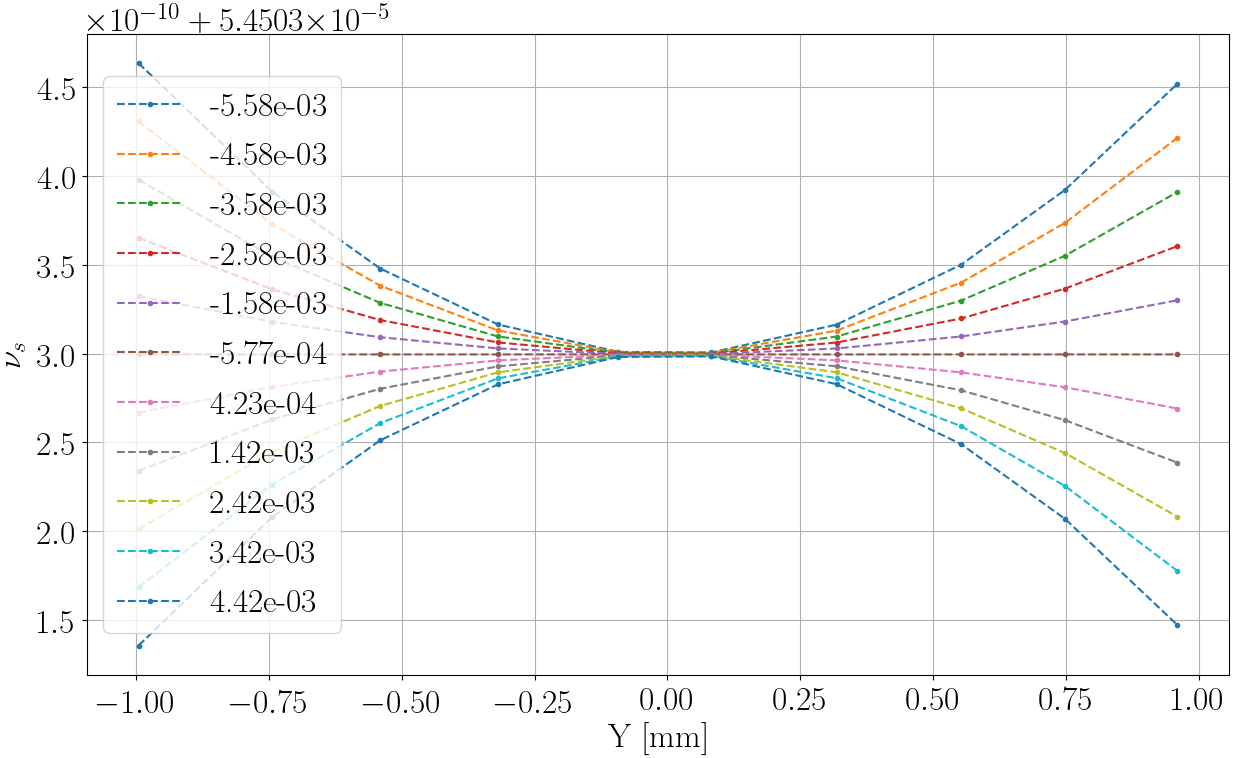
\includegraphics[width=\linewidth]{images/decoh_sim/spin_tune_vs_offset}
		\caption{Full range.\label{decoh:fig:full:ST_vs_y0_GSY}}
	\end{subfigure}
	\begin{subfigure}{\linewidth}
		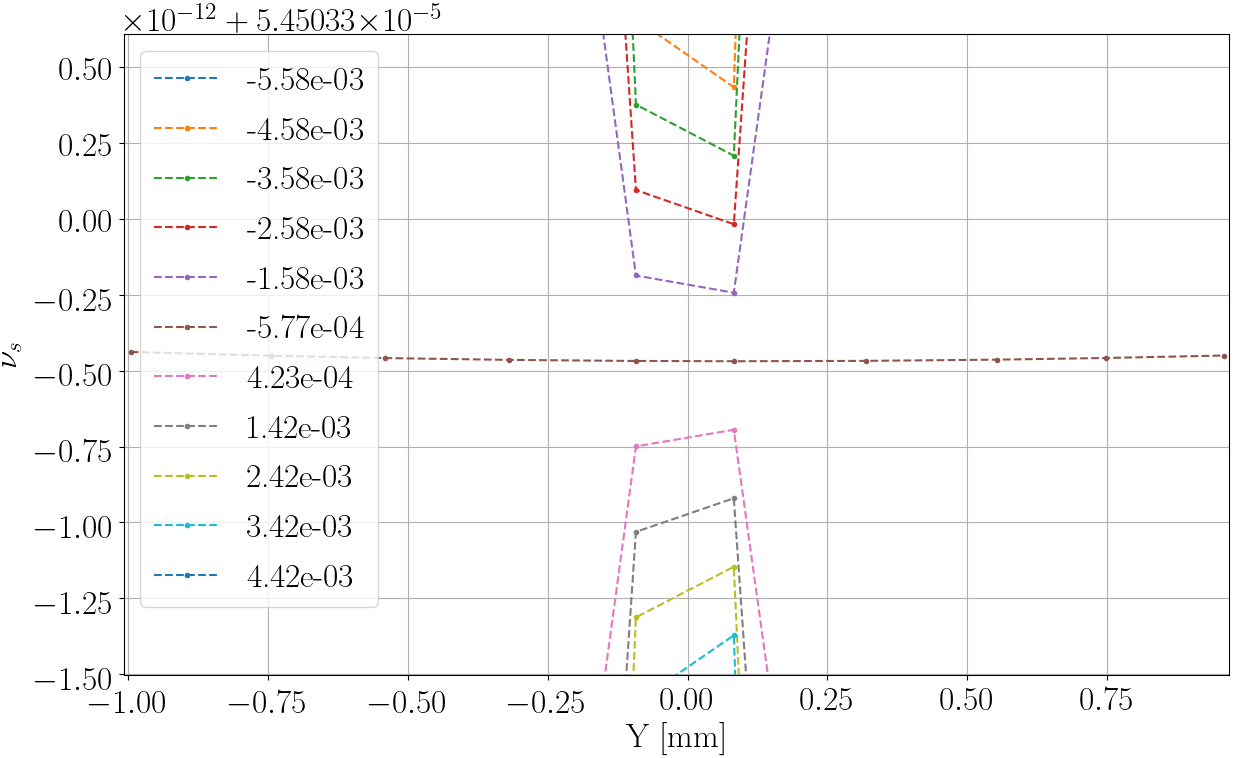
\includegraphics[width=\linewidth]{images/decoh_sim/spin_tune_vs_offset_zoom}
		\caption{Detalization.\label{decoh:fig:zoom:ST_vs_y0_GSY}}
	\end{subfigure}
	\caption{Spin tune $\nu_s$ as a function of the particle's vertical offset from the closed orbit.
          Color marks different $G_Y$ values.\label{decoh:fig:ST_vs_y0_GSY}}
\end{figure}

An equivalent dependence for the vetrical component of the ISA is shown
in Figure~\ref{decoh:fig:ny_vs_y0_GSY}. In Figure~\ref{decoh:fig:full:ny_vs_y0_GSY} we observe
that the ISA component behaves the same way as spin tune when $G_Y \rightarrow G_Y^0$.
Just as in the case of an ideal lattice, in Figure~\ref{decoh:fig:zoom:ny_vs_y0_GSY}
one can observe the presence of a linear term in $\nbar_y(y)$, insensitive to the sextupole fields.

\begin{figure}[h!]
	\centering
	\begin{subfigure}{\linewidth}
		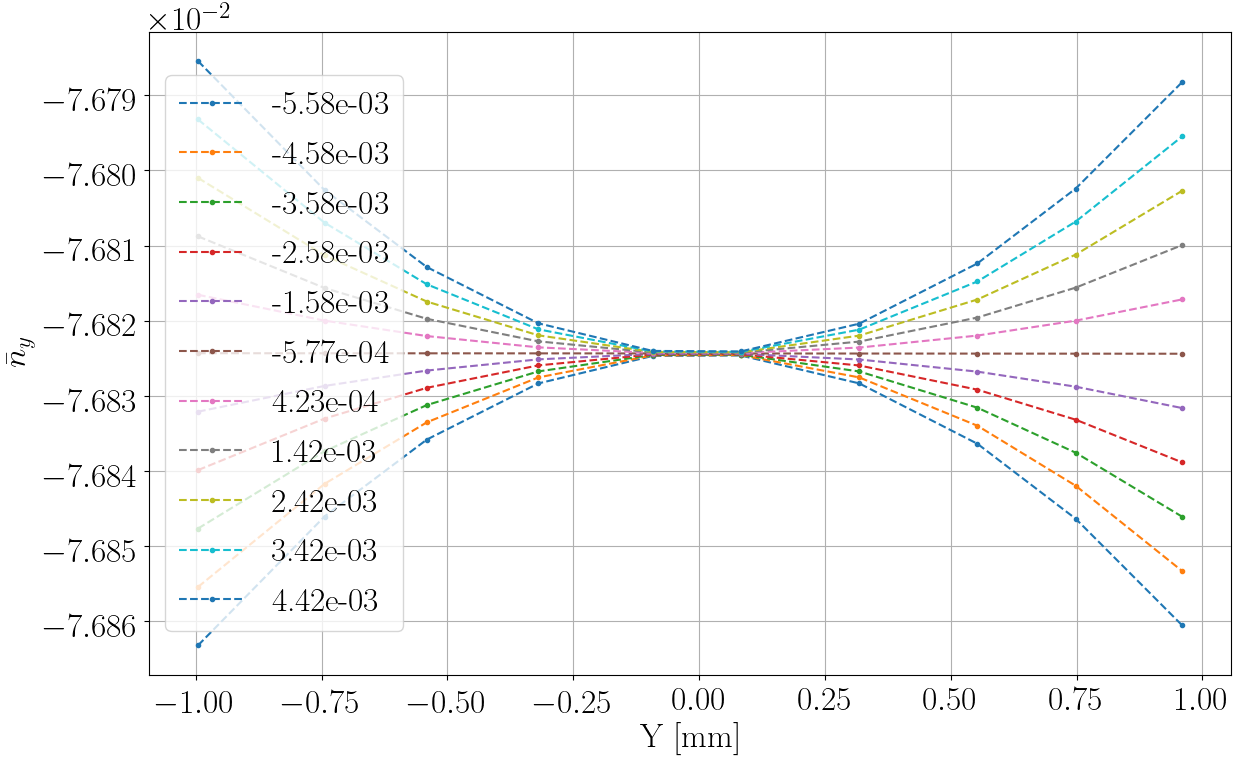
\includegraphics[width=\linewidth]{images/decoh_sim/ny_vs_offset}
		\caption{Full range.\label{decoh:fig:full:ny_vs_y0_GSY}}
	\end{subfigure}
	\begin{subfigure}{\linewidth}
		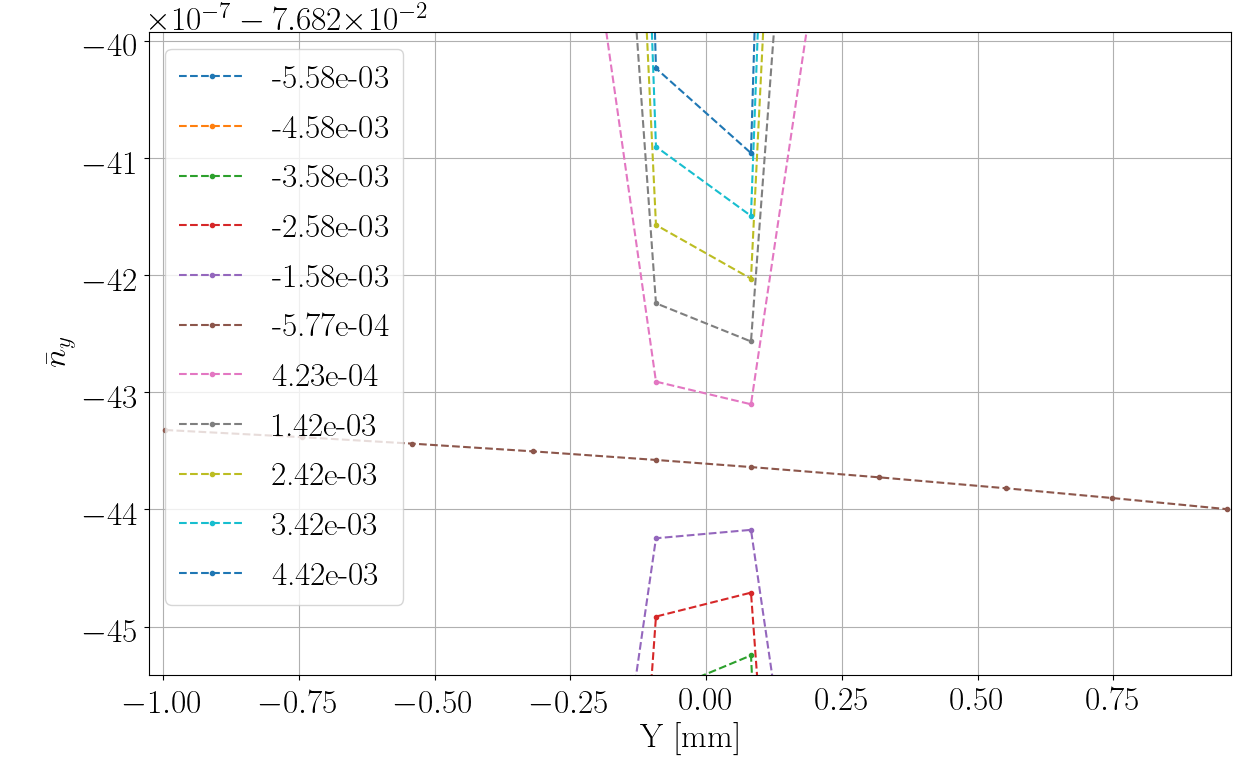
\includegraphics[width=\linewidth]{images/decoh_sim/ny_vs_offset_zoom}
		\caption{Detalization.\label{decoh:fig:zoom:ny_vs_y0_GSY}}
	\end{subfigure}
	\caption{Vertical component $\bar n_y$ of the invariant spin axis as a function of the particle's
          vertical offset from the closed orbit.
          Color marks different $G_Y$ values\label{decoh:fig:ny_vs_y0_GSY}}
\end{figure}

In the figures above, the values of spin tune and ISA were computed as univariate functions
of the vertical offset; all other phase space coordinates were set to reference values. While analyzing
the tracker data we noted that the ISA components (as well as spin tune) of a particle do not oscillate,
as one would expect from the figures, but remain nearly constant. We hypothesized that the $\nu_s$ and $\nbar$
dependencies on the vertical offset and ite derivative ($y'\equiv a$) compensate each other when the particle
moves along a real trajeoctory. On the next figures we depicted $\nu_s$, $\nbar$ at their true phase space
trajectories in the storage ring.

In Figure~\ref{decoh:fig:yb_traj} are depicted the particle trajectories in the $(Y,B)$ phase plane,
obtained in tracking the particles through the imperfect lattice.
\begin{figure}[h!]
	\centering
	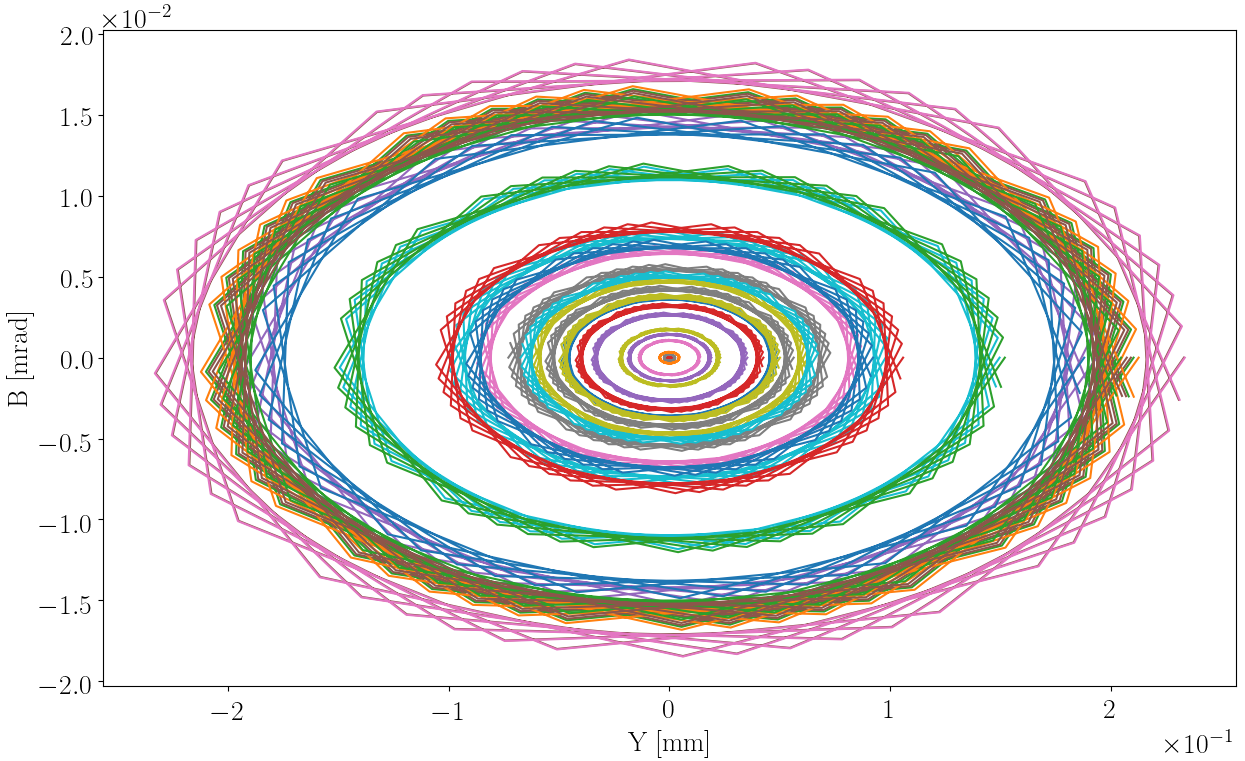
\includegraphics[width=\linewidth]{images/decoh_sim/YB-PHASE_SPACE_IMPERFECT_UNOPT}
	\caption{Particle trajectories in the $(Y,B)$ phase space.\label{decoh:fig:yb_traj}} 
\end{figure}

In Figures~\ref{decoh:fig:ST_on_traj}, \ref{decoh:fig:NX_on_traj}, \ref{decoh:fig:NY_on_traj}, and
\ref{decoh:fig:NZ_on_traj} are plotted, respectively: spin tune, the radial, vertical, and longitudinal
components of the ISA, computed at the trajectories plotted in Figure~\ref{decoh:fig:yb_traj}, in two cases:
\begin{enumerate*}[\itshape i\upshape)]
	\item sextupoles are turned off, and 
	\item GSY sextupoles are turned on.
\end{enumerate*}  

\begin{figure}[!h]
	\centering
	\begin{subfigure}{\linewidth}
		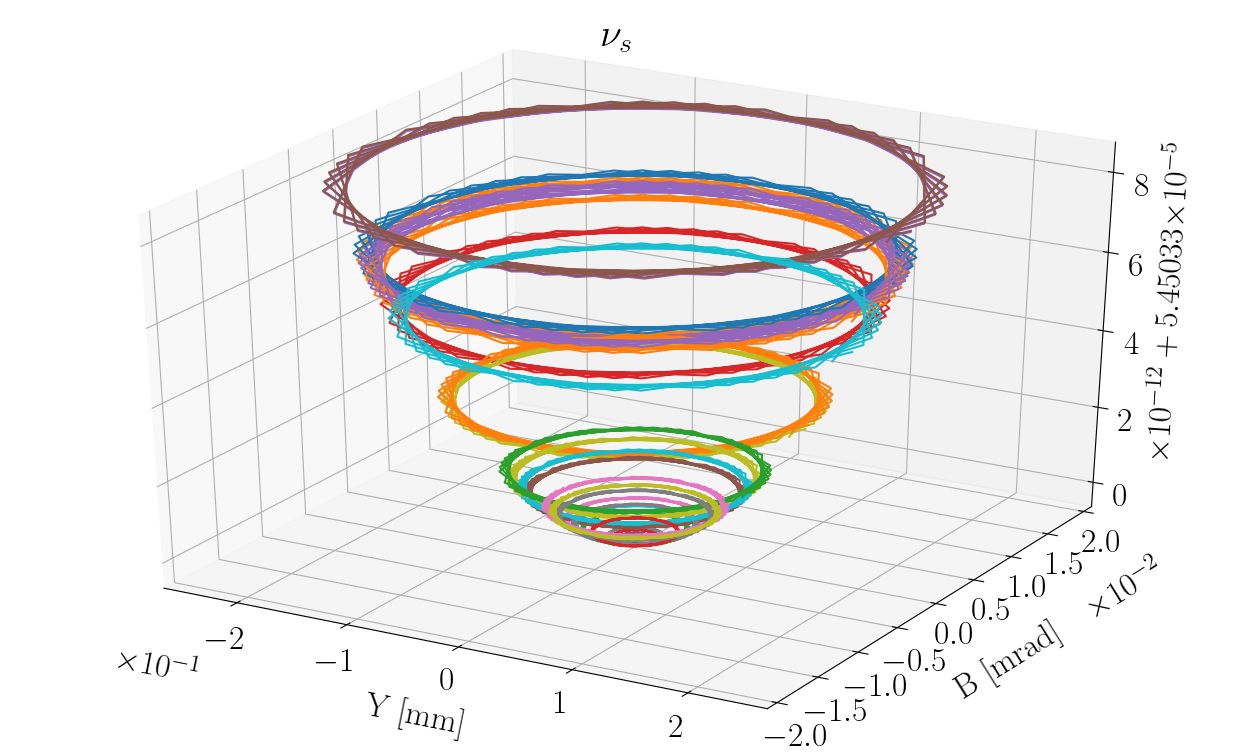
\includegraphics[width=\linewidth]{images/decoh_sim/ST_VS_YB_IMPERFECT_UNOPT}
		\caption{Sextupoles off.}
	\end{subfigure}
	\begin{subfigure}{\linewidth}
		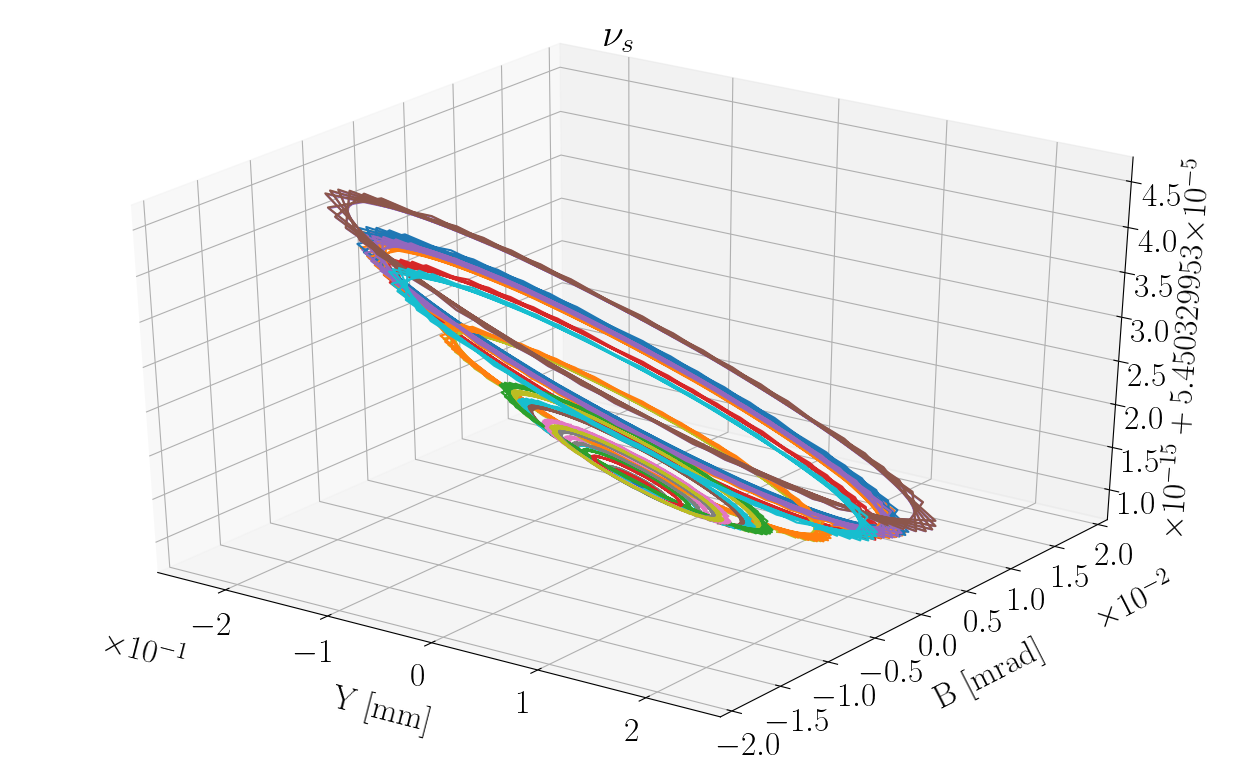
\includegraphics[width=\linewidth]{images/decoh_sim/ST_VS_YB_IMPERFECT_OPTIM}
		\caption{Sextupoles on.}
	\end{subfigure}
	\caption{Particle spin tunes computed at their trajectories
          in an imperfect FS lattice.\label{decoh:fig:ST_on_traj}}
\end{figure}

\begin{figure}[!h]
	\centering
	\begin{subfigure}{\linewidth}
		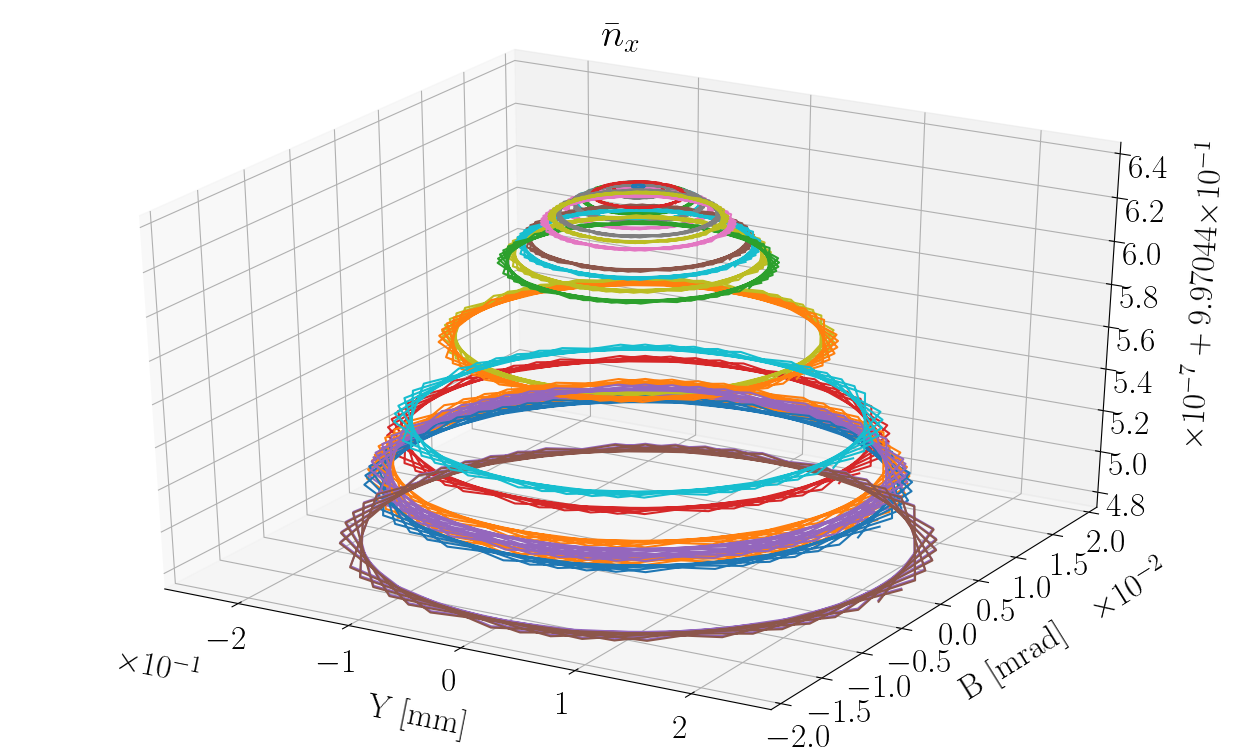
\includegraphics[width=\linewidth]{images/decoh_sim/NX_VS_YB_IMPERFECT_UNOPT}
		\caption{Sextupoles off.}
	\end{subfigure}
	\begin{subfigure}{\linewidth}
		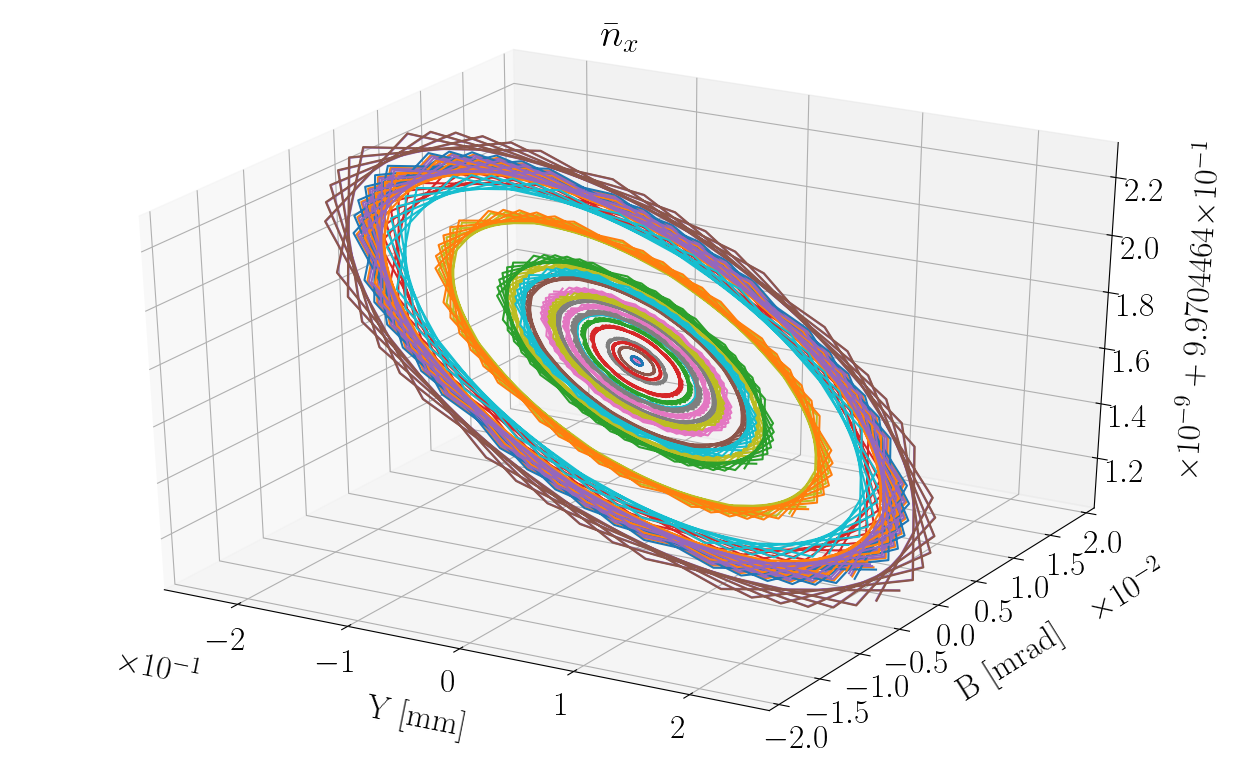
\includegraphics[width=\linewidth]{images/decoh_sim/NX_VS_YB_IMPERFECT_OPTIM}
		\caption{Sextupoles on.}
	\end{subfigure}
	\caption{Particle's radial ISA components computed at their trajectories
          in an imperfect FS lattice.\label{decoh:fig:NX_on_traj}}
\end{figure}

\begin{figure}[!h]
	\centering
	\begin{subfigure}{\linewidth}
		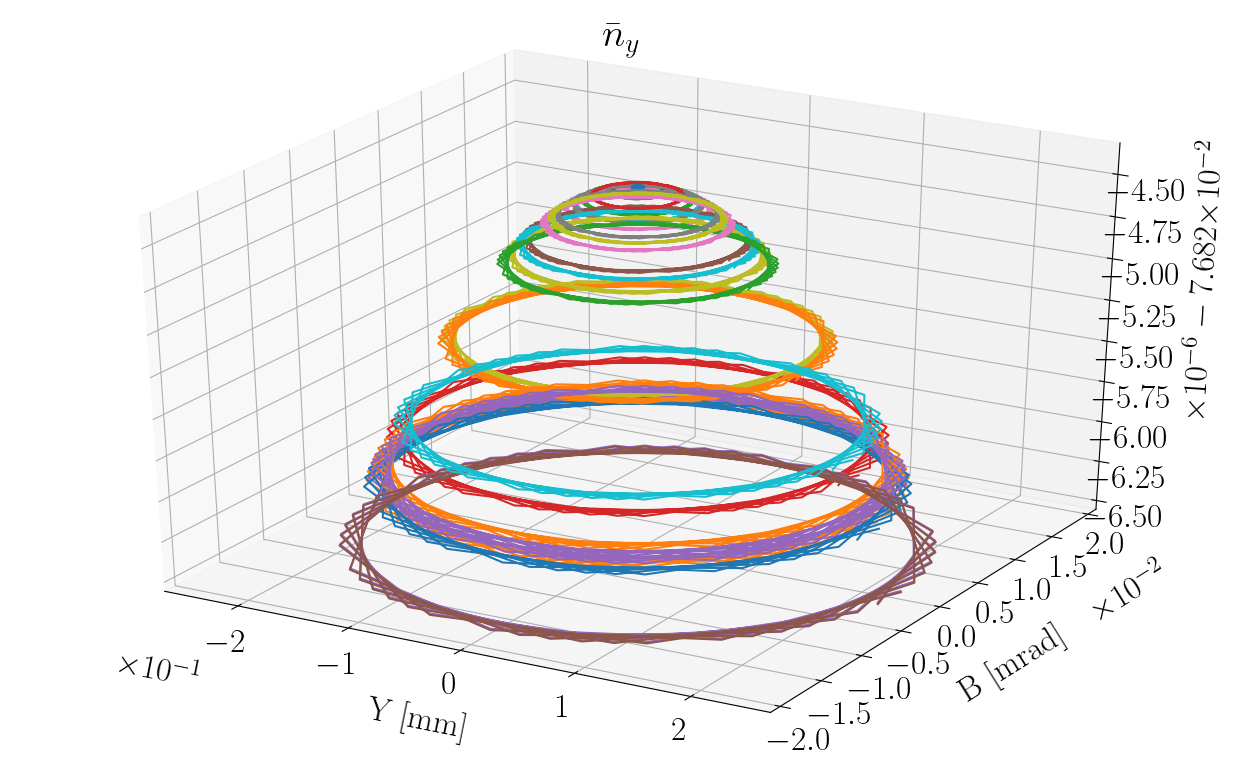
\includegraphics[width=\linewidth]{images/decoh_sim/NY_VS_YB_IMPERFECT_UNOPT}
		\caption{Sextupoles off.}
	\end{subfigure}
	\begin{subfigure}{\linewidth}
		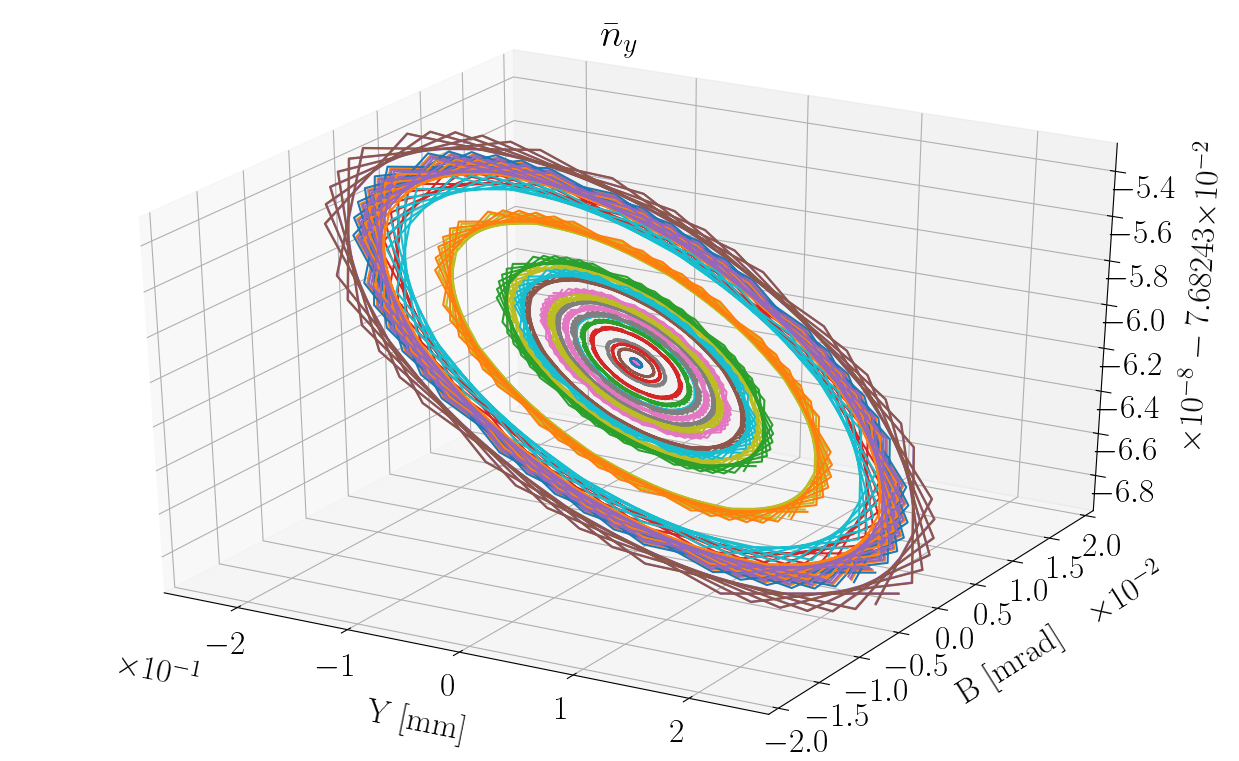
\includegraphics[width=\linewidth]{images/decoh_sim/NY_VS_YB_IMPERFECT_OPTIM}
		\caption{Sextupoles on.}
	\end{subfigure}
	\caption{Particle's vertical ISA components computed at their trajectories
          in an imperfect FS lattice.\label{decoh:fig:NY_on_traj}}
\end{figure}

\begin{figure}[!h]
	\centering
	\begin{subfigure}{\linewidth}
		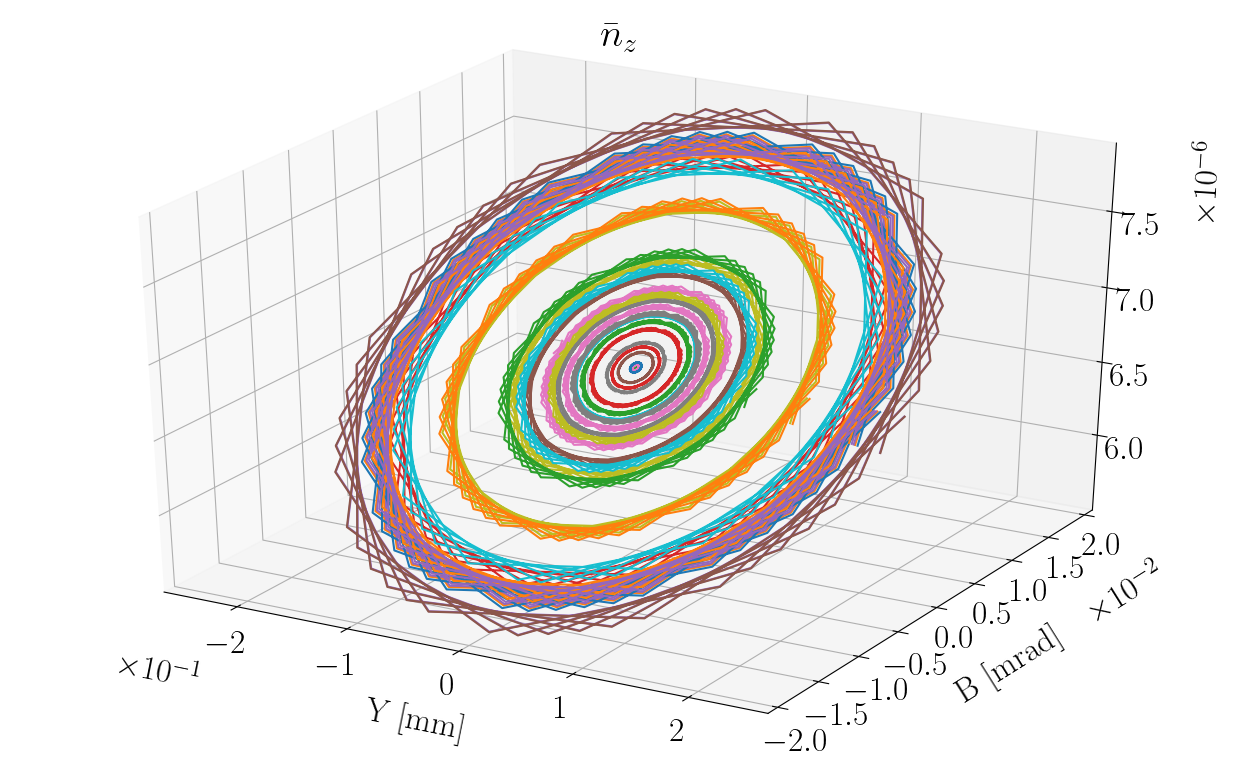
\includegraphics[width=\linewidth]{images/decoh_sim/NZ_VS_YB_IMPERFECT_UNOPT}
		\caption{Sextupoles off.}
	\end{subfigure}
	\begin{subfigure}{\linewidth}
		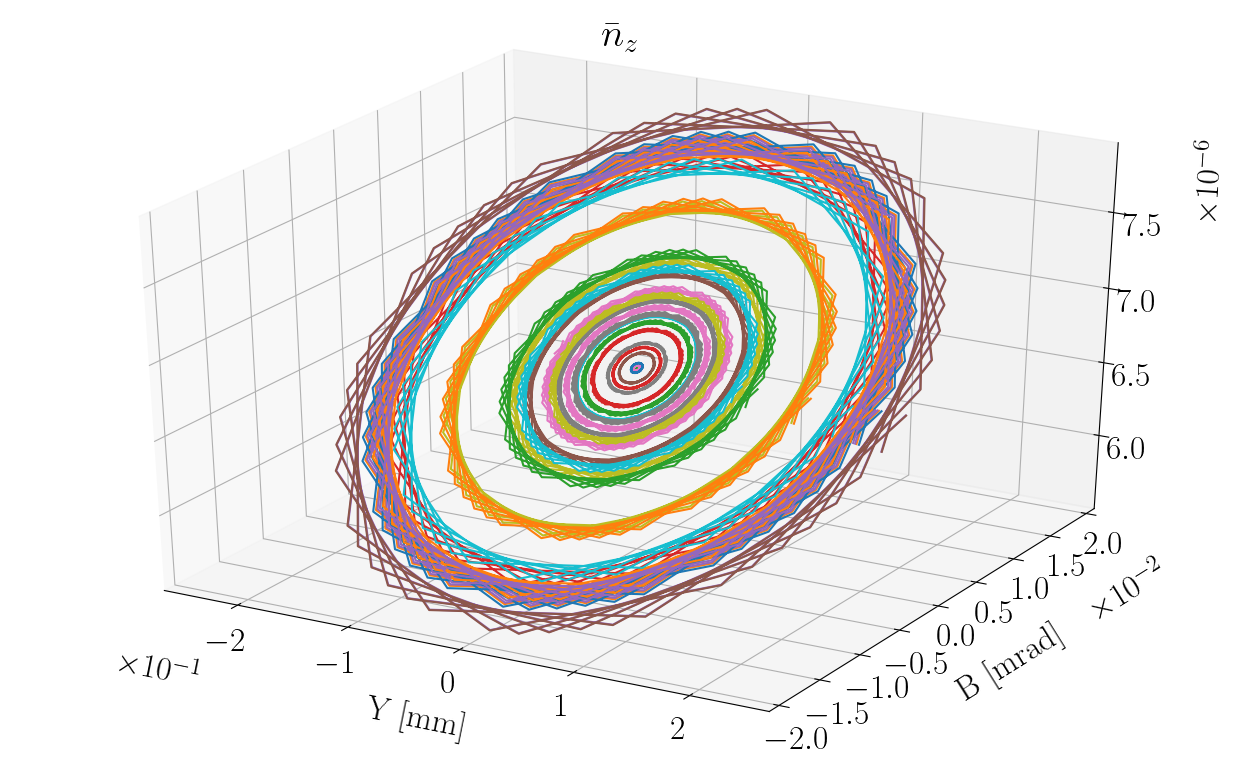
\includegraphics[width=\linewidth]{images/decoh_sim/NZ_VS_YB_IMPERFECT_OPTIM}
		\caption{Sextupoles on.}
	\end{subfigure}
	\caption{Particle's longitudinal ISA components computed at their trajectories
          in an imperfect FS lattice.\label{decoh:fig:NZ_on_traj}}
\end{figure}

From the analysis of the figures, we can gather the following:
\begin{enumerate}
\item in the sextupoles-off case, both $\nu_s$ and the direction of $\nbar$ are mostly (to the
  linear Taylor expansion term) fixed by the value of the particle's transverse emittance;
\item in the sextupoles-on case, the mean levels of $\nu_s$ and $\nbar$ of different particles come
  together, and the betatron motion effect, related to the presence of a linear Taylor expansion term,
  becomes apparent.
\end{enumerate}
Hence, Figures~\ref{decoh:fig:NX_on_traj} and~\ref{decoh:fig:NY_on_traj} are evidence that not only are the
\textbf{frequencies} but also the \textbf{directions} of the beam particles' spin precession angular
velocity vectors are equalized when sextupole fields are used to suppress spin decoherence. The
longitudinal component of the ISA is insensitive to the sextupole fields, as evicdenced
by Figure~\ref{decoh:fig:NZ_on_traj}.

In Figure~\ref{decoh:fig:nbar_vs_ST} are shown the dependencies of the radial and vertical ISA components'
mean levels on the particle's mean spin tune level. Based on this figure, we conclude
in section~\ref{sec:spin_stune_traj_equ:B_form} that particles having equal effective Lorentz factor values
are equivalent in terms of their spin dynamics in the general (direction and magnitude of the spin precession
angular velocity vector) sense.~\footnote{At least this seems to be true when operating
  in the frozen spin regime.}
\begin{figure}[!h]
	\centering
	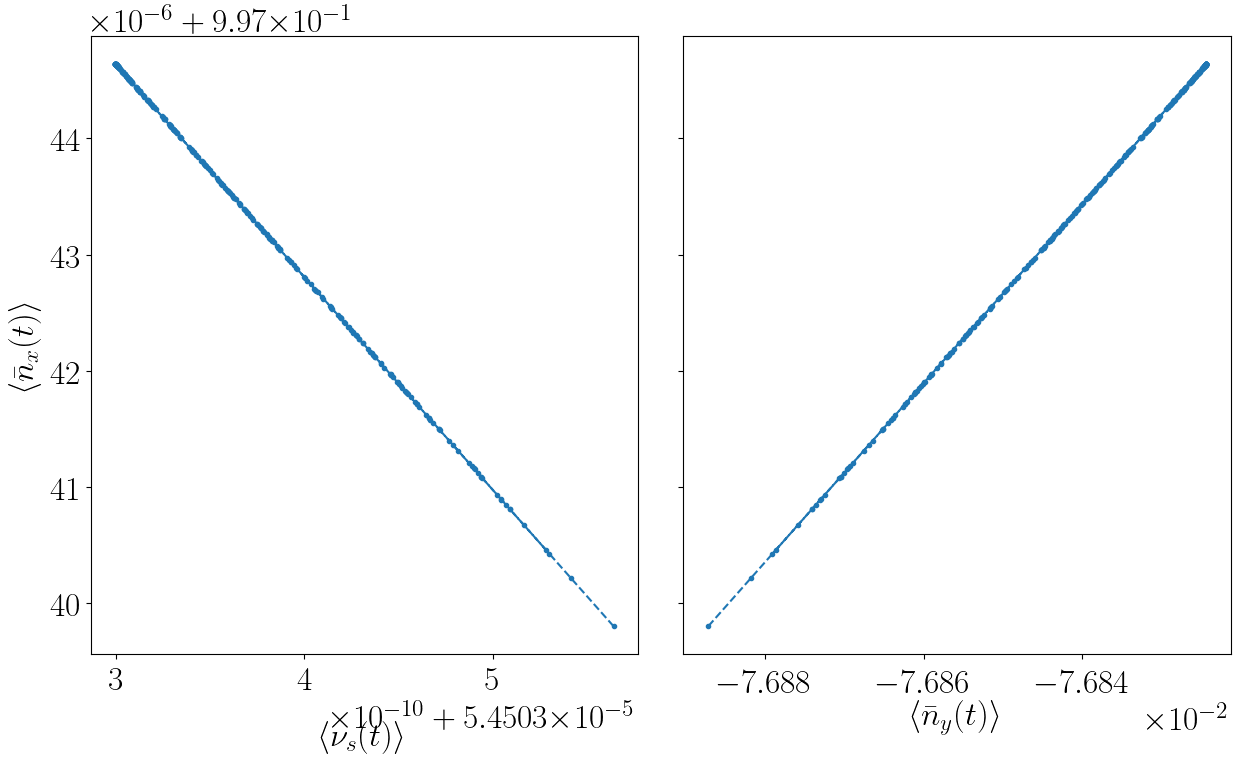
\includegraphics[width=\linewidth]{images/decoh_sim/mean_n_bar_vs_spin_tune}
	\caption{Mean level of the radial and vertical ISA components versus the correcponding
          value of spin tune.\label{decoh:fig:nbar_vs_ST}}
\end{figure}

\subsection{Analysis of the sextupole spin decoherence suppression mechanism}\label{sec:sext_decoh_suppression_effect_analysis}
From equations~\eqref{eq:spin_tune_vs_gamma} and~\eqref{eq:EquLevMom_shift}, the dependence of spin tune of the
particle equilibrium energy can be expressed as:
\[
\nu_s = G\gamma_0 + G\frac{\gamma_0^2-1}{\gamma_0}\cdot C_0\cdot f_1(\epsilon_x, \epsilon_y, Q_x, Q_y)+ G\frac{\gamma_0^2-1}{\gamma_0}\cdot C_0\cdot f_2(\alpha_1, \avg{\Delta K/K}^2),
\]
where $C_0$ is a constant, $f_1$ and $f_2$ are defined in equation~\eqref{eq:EquLevMom_shift}.

Since a betatron-oscillating particle does also synchrotron oscillations, the effct of sextupole fields on it
is a superposition of effects. A particle injected onto the reference orbit, but having an initial energy
offset, does only synchrotron oscillations. Consequently, sextupole fields affect its spin tune by only
modifying the momentum compaction factor, i.e. $f_2$.

In view of that, we carried out a simulation in which we consecutively injected two beams of 30 particles:
in the first one, the D-bunch, particles were distributed as $\delta\sim N(0, 0.5\cdot 10^{-6})$, 
in the second one, the Y-bunch, as $y\sim N(0, 0.5)$ mm. All the other phase space coordinates were initially
set to zero.

The bunches were injected into the ideal FS lattice in order to exclude effects associated with perturbations
of non-reference orbits. For the D-bunch, only the GSD sextupoles were turned on; for the Y-bunch -- GSY. The
sextupole gradients were varied $\pm 5\cdot 10^{-3}$ of the corresponding family's optimal gradient value.

Spin tracking was done for $1.2\cdot 10^6$ turns, data were recorded every 800 turns.

In Figure~\ref{fig:long_PS_sext_settings} are plotted the particles' longitudinal phase space portraits. 
We see that the D-bunch phase portraits are practically all centered at the same point,~\footnote{When zooming 	in, one can see that the ellipse centers are slightly different, but this difference is insensitive to
	the sextupole gradient value, and most likely is the result of finite statistics.} and that their 
emittances do not change when the sextupole strength is varied.

At the same time, the Y-bunch phase portraits vary with the sextupole field strength. We observe that the 
the ellipse centers (i.e. the equilibrium energy levels) are the most compressed at a gradient value that is
\textbf{not} optimal (the phase portraits for the latter are drawn in the middle panel). This observation
was what motivated us to try to inject the D-bunch in the first place. We explain this observation by the
superposition of the orbit length and momentum compaction factor effects.

\begin{figure}[h]
	\centering
	\begin{subfigure}{\linewidth}
		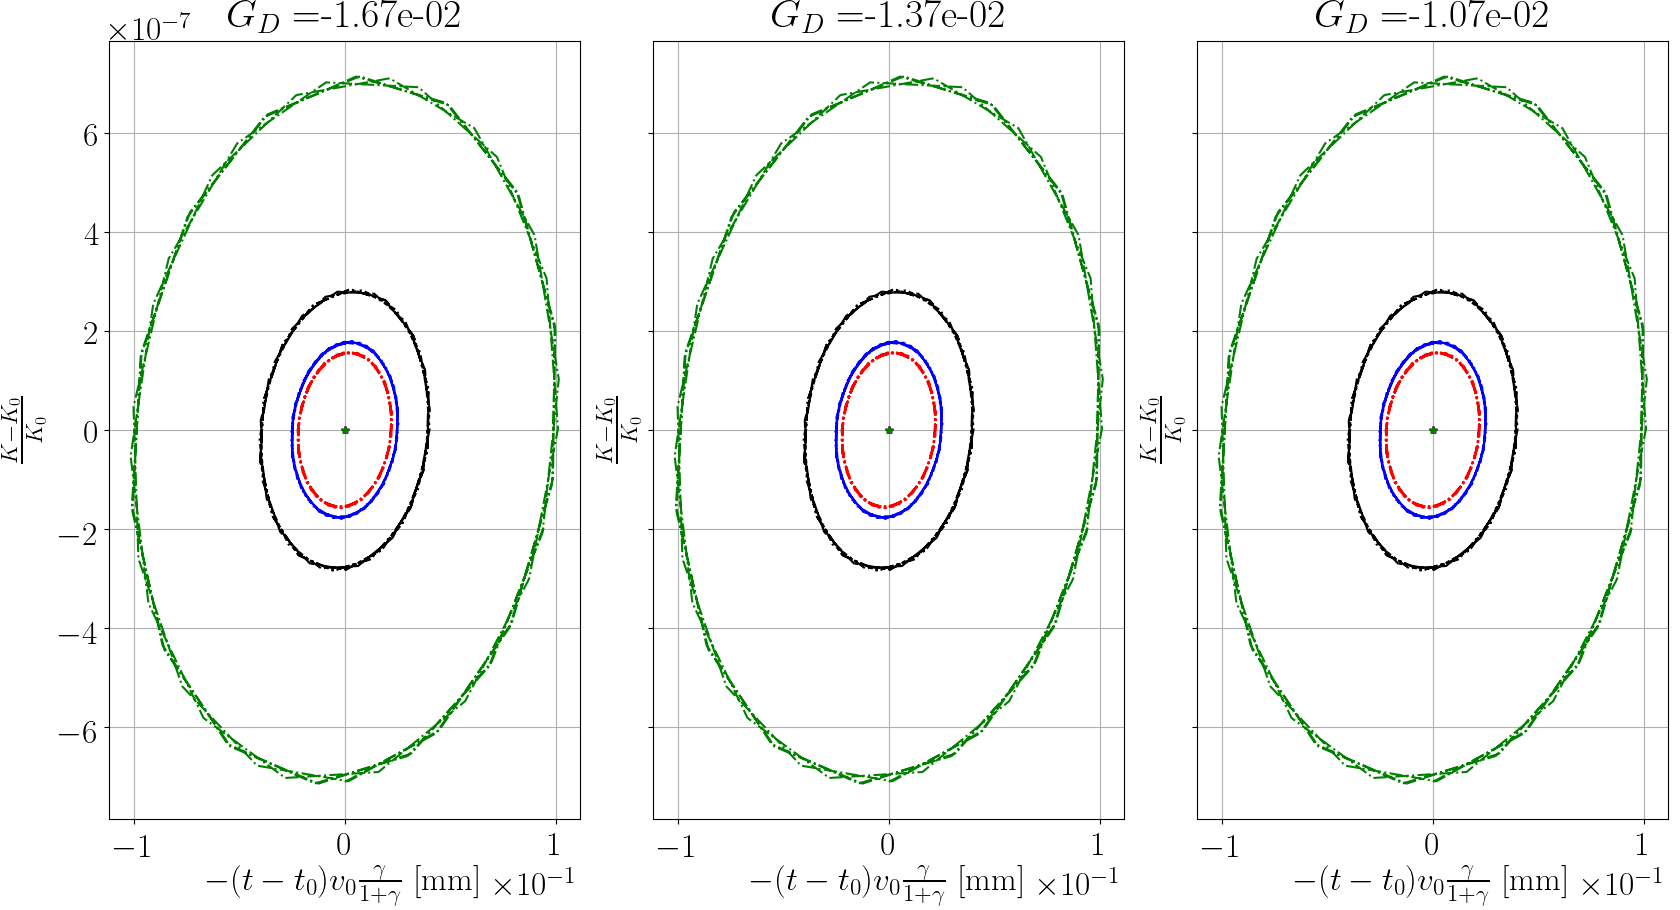
\includegraphics[width=\linewidth]{images/decoh_sim/propdef/long_phase_space_for_sext_settings_D}
		\caption{D-bunch phase portraits.}
	\end{subfigure}
	\begin{subfigure}{\linewidth}
		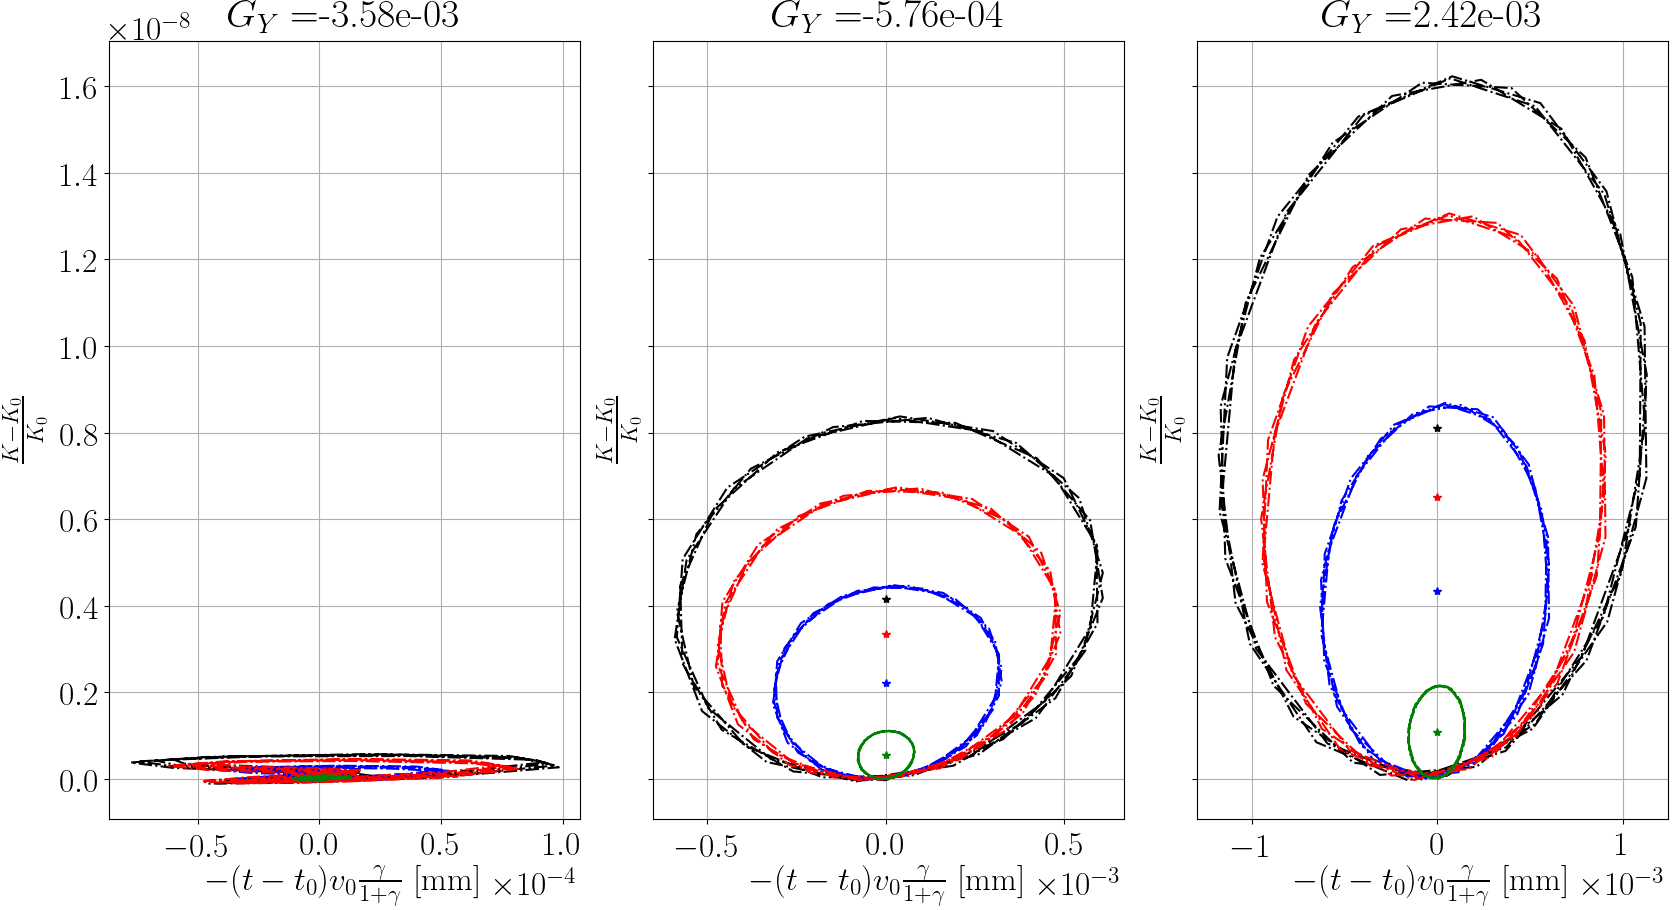
\includegraphics[width=\linewidth]{images/decoh_sim/propdef/long_phase_space_for_sext_settings_Y}
		\caption{Y-bunch phase portraits.}
	\end{subfigure}
	\caption{Longitudinal phase space particle portraits. Asterisks mark the ellipse centers.
		Colors mark trajectories of particles with differing initial vertical offset from the reference orbit.\label{fig:long_PS_sext_settings}}
\end{figure}

For a more thorough analysis of the sextupoel field effects on the functions $f_1$ and $f_2$ we plotted the
dependencies of the particles' mean spin tune levels on their equilibrium energy levels at different
sextupole field strengths (Figure~\ref{fig:ST_vs_dkok_for_sext_strenghts}). One can see from the figure 
that the point distribution density in the D-bunch plot does not vary with the gradient value; the only thing 
that changes is the functional dependence of spin tune on the equilibrium energy level, as is expected from
the functional form of $f_2$ (cf. section~\ref{chpt1:FS-methods:effective-Lorentz-factor}). Hence, the 
signature of the sextupole field's momentum compaction effect is the change in the functional form of
 $\avg{\nu_s} = f(\avg{\Delta K/K})$.

In the Y-bunch plot one observes two effects: both the point distribution density (i.e. the beam's longitudinal emittance) and the functional form of $\avg{\nu_s}(\avg{\Delta K/K})$ change.

\begin{figure}[h]
	\centering
	\begin{subfigure}{\linewidth}
		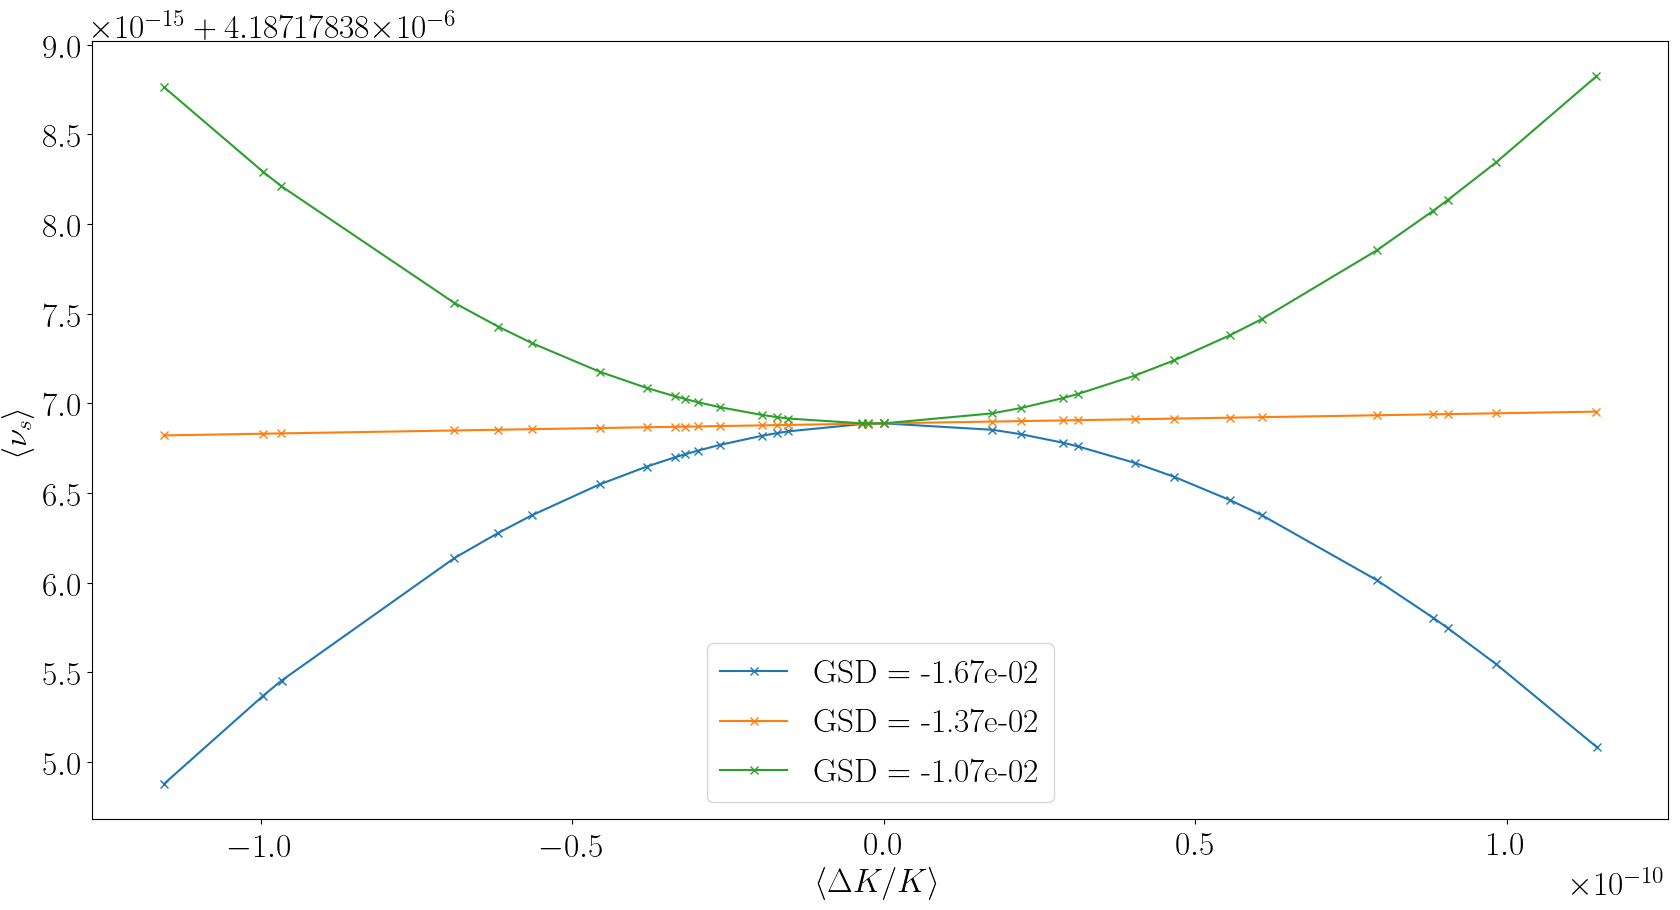
\includegraphics[width=\linewidth]{images/decoh_sim/propdef/stune_vs_dkok_SS_D}
		\caption{For the D-bunch.}
	\end{subfigure}
	\begin{subfigure}{\linewidth}
		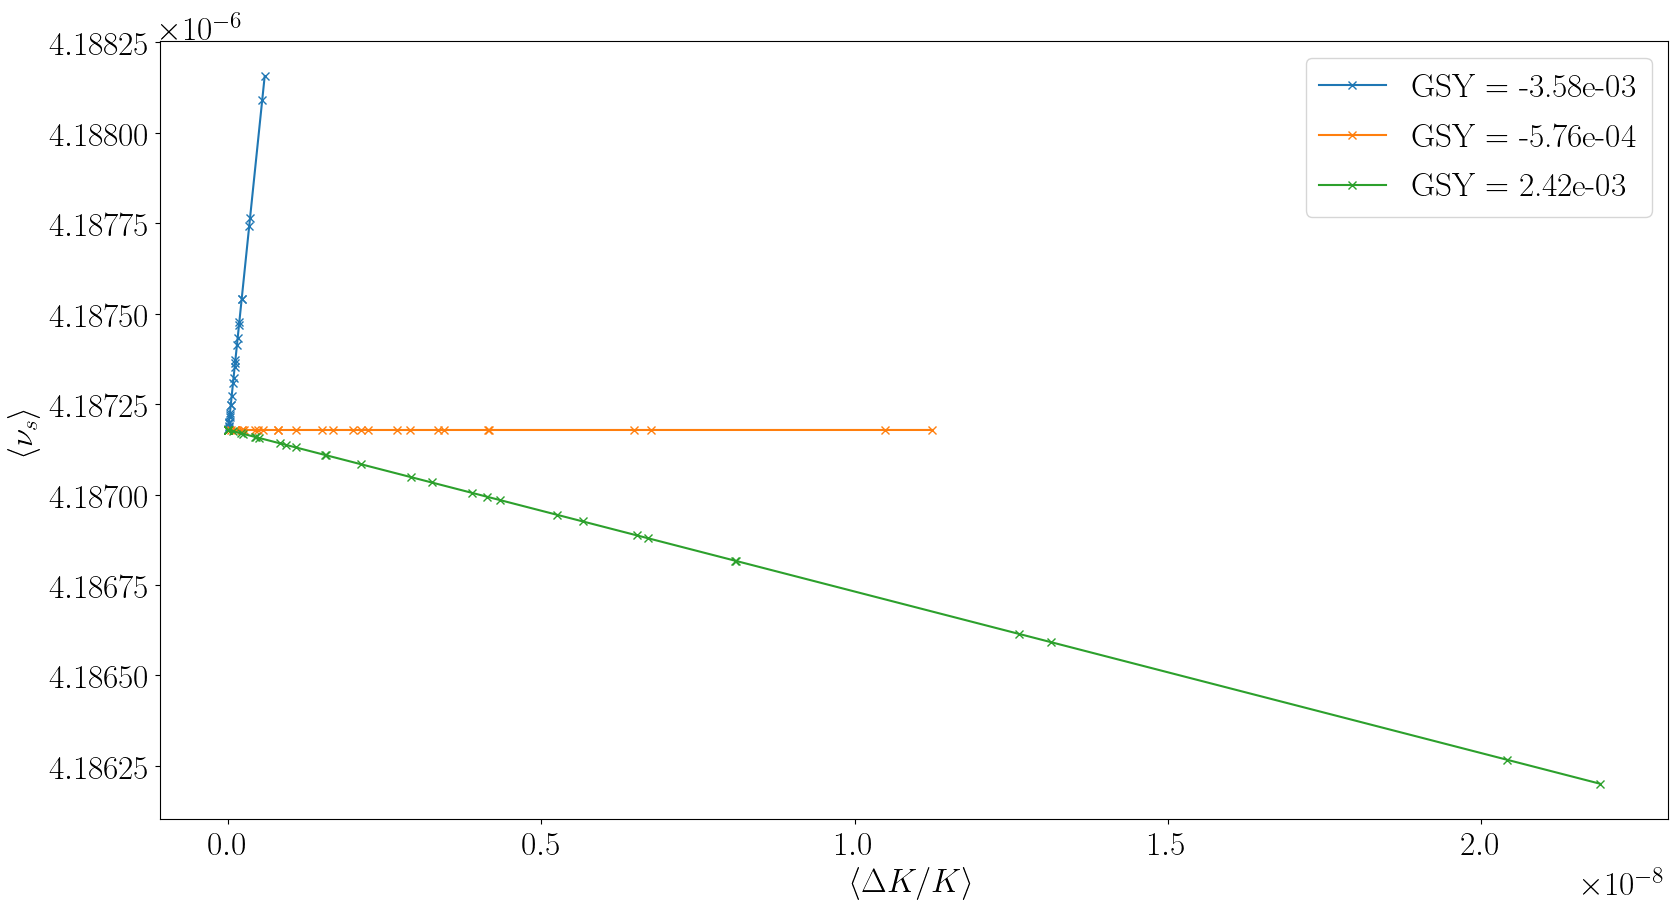
\includegraphics[width=\linewidth]{images/decoh_sim/propdef/stune_vs_dkok_SS_Y}
		\caption{For the Y-bunch.}
	\end{subfigure}
	\caption{Particle mean spin tune level as a function of its equilibrium level energy at different sextupole strengths.\label{fig:ST_vs_dkok_for_sext_strenghts}}
\end{figure}

\paragraph{Conclusion:} The simulation confirms statements~\eqref{eq:Sext_compaction_effect} and~\eqref{eq:Sext_OL_effect}.
